% Options for packages loaded elsewhere
\PassOptionsToPackage{unicode}{hyperref}
\PassOptionsToPackage{hyphens}{url}
%
\documentclass[
  american,
  man]{apa7}
\usepackage{lmodern}
\usepackage{amssymb,amsmath}
\usepackage{ifxetex,ifluatex}
\ifnum 0\ifxetex 1\fi\ifluatex 1\fi=0 % if pdftex
  \usepackage[T1]{fontenc}
  \usepackage[utf8]{inputenc}
  \usepackage{textcomp} % provide euro and other symbols
\else % if luatex or xetex
  \usepackage{unicode-math}
  \defaultfontfeatures{Scale=MatchLowercase}
  \defaultfontfeatures[\rmfamily]{Ligatures=TeX,Scale=1}
\fi
% Use upquote if available, for straight quotes in verbatim environments
\IfFileExists{upquote.sty}{\usepackage{upquote}}{}
\IfFileExists{microtype.sty}{% use microtype if available
  \usepackage[]{microtype}
  \UseMicrotypeSet[protrusion]{basicmath} % disable protrusion for tt fonts
}{}
\makeatletter
\@ifundefined{KOMAClassName}{% if non-KOMA class
  \IfFileExists{parskip.sty}{%
    \usepackage{parskip}
  }{% else
    \setlength{\parindent}{0pt}
    \setlength{\parskip}{6pt plus 2pt minus 1pt}}
}{% if KOMA class
  \KOMAoptions{parskip=half}}
\makeatother
\usepackage{xcolor}
\IfFileExists{xurl.sty}{\usepackage{xurl}}{} % add URL line breaks if available
\IfFileExists{bookmark.sty}{\usepackage{bookmark}}{\usepackage{hyperref}}
\hypersetup{
  pdftitle={Pilot Study 1},
  pdfauthor={Blinded1, Blinded2, Blinded1, \& Blinded1},
  pdflang={en-US},
  pdfkeywords={keywords},
  hidelinks,
  pdfcreator={LaTeX via pandoc}}
\urlstyle{same} % disable monospaced font for URLs
\usepackage{graphicx,grffile}
\makeatletter
\def\maxwidth{\ifdim\Gin@nat@width>\linewidth\linewidth\else\Gin@nat@width\fi}
\def\maxheight{\ifdim\Gin@nat@height>\textheight\textheight\else\Gin@nat@height\fi}
\makeatother
% Scale images if necessary, so that they will not overflow the page
% margins by default, and it is still possible to overwrite the defaults
% using explicit options in \includegraphics[width, height, ...]{}
\setkeys{Gin}{width=\maxwidth,height=\maxheight,keepaspectratio}
% Set default figure placement to htbp
\makeatletter
\def\fps@figure{htbp}
\makeatother
\setlength{\emergencystretch}{3em} % prevent overfull lines
\providecommand{\tightlist}{%
  \setlength{\itemsep}{0pt}\setlength{\parskip}{0pt}}
\setcounter{secnumdepth}{-\maxdimen} % remove section numbering
% Make \paragraph and \subparagraph free-standing
\ifx\paragraph\undefined\else
  \let\oldparagraph\paragraph
  \renewcommand{\paragraph}[1]{\oldparagraph{#1}\mbox{}}
\fi
\ifx\subparagraph\undefined\else
  \let\oldsubparagraph\subparagraph
  \renewcommand{\subparagraph}[1]{\oldsubparagraph{#1}\mbox{}}
\fi
% Manuscript styling
\usepackage{upgreek}
\captionsetup{font=singlespacing,justification=justified}

% Table formatting
\usepackage{longtable}
\usepackage{lscape}
% \usepackage[counterclockwise]{rotating}   % Landscape page setup for large tables
\usepackage{multirow}		% Table styling
\usepackage{tabularx}		% Control Column width
\usepackage[flushleft]{threeparttable}	% Allows for three part tables with a specified notes section
\usepackage{threeparttablex}            % Lets threeparttable work with longtable

% Create new environments so endfloat can handle them
% \newenvironment{ltable}
%   {\begin{landscape}\centering\begin{threeparttable}}
%   {\end{threeparttable}\end{landscape}}
\newenvironment{lltable}{\begin{landscape}\centering\begin{ThreePartTable}}{\end{ThreePartTable}\end{landscape}}

% Enables adjusting longtable caption width to table width
% Solution found at http://golatex.de/longtable-mit-caption-so-breit-wie-die-tabelle-t15767.html
\makeatletter
\newcommand\LastLTentrywidth{1em}
\newlength\longtablewidth
\setlength{\longtablewidth}{1in}
\newcommand{\getlongtablewidth}{\begingroup \ifcsname LT@\roman{LT@tables}\endcsname \global\longtablewidth=0pt \renewcommand{\LT@entry}[2]{\global\advance\longtablewidth by ##2\relax\gdef\LastLTentrywidth{##2}}\@nameuse{LT@\roman{LT@tables}} \fi \endgroup}

% \setlength{\parindent}{0.5in}
% \setlength{\parskip}{0pt plus 0pt minus 0pt}

% Overwrite redefinition of paragraph and subparagraph by the default LaTeX template
% See https://github.com/crsh/papaja/issues/292
\makeatletter
\renewcommand{\paragraph}{\@startsection{paragraph}{4}{\parindent}%
  {0\baselineskip \@plus 0.2ex \@minus 0.2ex}%
  {-1em}%
  {\normalfont\normalsize\bfseries\itshape\typesectitle}}

\renewcommand{\subparagraph}[1]{\@startsection{subparagraph}{5}{1em}%
  {0\baselineskip \@plus 0.2ex \@minus 0.2ex}%
  {-\z@\relax}%
  {\normalfont\normalsize\itshape\hspace{\parindent}{#1}\textit{\addperi}}{\relax}}
\makeatother

% \usepackage{etoolbox}
\makeatletter
\patchcmd{\HyOrg@maketitle}
  {\section{\normalfont\normalsize\abstractname}}
  {\section*{\normalfont\normalsize\abstractname}}
  {}{\typeout{Failed to patch abstract.}}
\patchcmd{\HyOrg@maketitle}
  {\section{\protect\normalfont{\@title}}}
  {\section*{\protect\normalfont{\@title}}}
  {}{\typeout{Failed to patch title.}}
\makeatother

\usepackage{xpatch}
\makeatletter
\xapptocmd\appendix
  {\xapptocmd\section
    {\addcontentsline{toc}{section}{\appendixname\ifoneappendix\else~\theappendix\fi\\: #1}}
    {}{\InnerPatchFailed}%
  }
{}{\PatchFailed}
\keywords{keywords\newline\indent Word count: TBC}
\DeclareDelayedFloatFlavor{ThreePartTable}{table}
\DeclareDelayedFloatFlavor{lltable}{table}
\DeclareDelayedFloatFlavor*{longtable}{table}
\makeatletter
\renewcommand{\efloat@iwrite}[1]{\immediate\expandafter\protected@write\csname efloat@post#1\endcsname{}}
\makeatother
\usepackage{csquotes}
\usepackage[titles]{tocloft}
\cftpagenumbersoff{figure}
\renewcommand{\cftfigpresnum}{\itshape\figurename\enspace}
\renewcommand{\cftfigaftersnum}{.\space}
\setlength{\cftfigindent}{0pt}
\setlength{\cftafterloftitleskip}{0pt}
\settowidth{\cftfignumwidth}{Figure 10.\qquad}
\cftpagenumbersoff{table}
\renewcommand{\cfttabpresnum}{\itshape\tablename\enspace}
\renewcommand{\cfttabaftersnum}{.\space}
\setlength{\cfttabindent}{0pt}
\setlength{\cftafterloftitleskip}{0pt}
\settowidth{\cfttabnumwidth}{Table 10.\qquad}
\raggedbottom
\ifxetex
  % Load polyglossia as late as possible: uses bidi with RTL langages (e.g. Hebrew, Arabic)
  \usepackage{polyglossia}
  \setmainlanguage[variant=american]{english}
\else
  \usepackage[shorthands=off,main=american]{babel}
\fi

\title{Pilot Study 1}
\author{Blinded\textsuperscript{1}, Blinded\textsuperscript{2}, Blinded\textsuperscript{1}, \& Blinded\textsuperscript{1}}
\date{}


\shorttitle{Moral Dilution}

\authornote{

Correspondence concerning this article should be addressed to Blinded, Blinded. E-mail: Blinded

}

\affiliation{\vspace{0.5cm}\textsuperscript{1} Blinded\\\textsuperscript{2} Blinded}

\abstract{%
Six studies etc.
}



\begin{document}
\maketitle

\hypertarget{pilot-study-1}{%
\section{Pilot Study 1}\label{pilot-study-1}}

The aim of this pilot study was to develop and test materials that could be used to study the dilution effect for moral characters. We developed diagnostic and non-diagnostic character descriptions. We hypothesized that moral evaluations of the diagnostic descriptions would be more severe (more immoral) than for the non-diagnostic descriptions.

\hypertarget{pilot-study-1-method}{%
\subsection{Pilot Study 1: Method}\label{pilot-study-1-method}}

\hypertarget{pilot-1-participants-and-design}{%
\subsubsection{Pilot 1: Participants and design}\label{pilot-1-participants-and-design}}

The pilot study was a within-subjects design. The independent variable was description type with two levels, \emph{diagnostic} and \emph{non-diagnostic}. We used two dependent variables. The first dependent variable was the four item moral perception scale (MPS-4), participants rated the characters on four dimensions using 7-point bipolar scales. The dimensions and scale endpoints were: Bad-Good, Immoral-Moral, Violent-Peaceful, Merciless-Empathetic, this showed excellent reliability, \(\alpha\) = 0.93. The second dependent variable was a single item moral perception measure (MM-1) which consisted of a 100-point slider ranging from 0 = \emph{Very Immoral} to 100 = \emph{Very Moral}. Both dependent variables were taken from Walker et al.~(2021).

A total sample of 235 (89 female, 142 male, 1 non-binary, 1 prefer not to say; \emph{M}\textsubscript{age} = 36.45, min = 20, max = 72, \emph{SD} = 10.23) started the survey. Participants were recruited from MTurk.

We removed participants who failed both manipulation checks (\emph{n} = 23), leaving a total sample of 212 participants (80 female, 128 male, 1 non-binary, 1 prefer not to say; \emph{M}\textsubscript{age} = 36.63, min = 20, max = 72, \emph{SD} = 10.34).

\hypertarget{pilot-1-procedure-and-materials}{%
\subsubsection{Pilot 1: Procedure and materials}\label{pilot-1-procedure-and-materials}}

Data were collected using an online questionnaire presented with Qualtrics (www.qualtrics.com). Participants were presented with descriptions of six characters.

Moral character descriptions were developed by combining descriptions relating to three different moral foundations. These descriptions were adapted from the items of the extended character morality questionnaire (Grizzard et al., 2020). A sample description reads: \emph{Imagine a person named Sam. Throughout their life they have been known to be cruel, act unfairly, and to betray their own group}. Full text of these descriptions can be found in the supplementary materials.

We developed neutral descriptions that included information relating to physical appearance/attributes, hobbies/activities, and family information, e.g., \emph{Imagine a person named Jackie. They have red hair, play tennis four times a month, and have one older sibling and one younger sibling}.

Character descriptions did not specify the gender of the charcters, and all characters had names that could be either male or female (Sam, Robin, Francis, Alex, Jackie, Charlie). All participants read six descriptions, four moral descriptions and two neutral. Pilot Study 1 was pre-registered at \color{blue}\url{https://aspredicted.org/3VK_8FD}\color{black}.

\hypertarget{pilot-1-results}{%
\subsection{Pilot 1: Results}\label{pilot-1-results}}

The means and standard deviations for MPS-4 for each scenario are as follows:
\emph{Sam} (diagnostic),
\emph{M}\textsubscript{MPS-4} = 4.35, \emph{SD}\textsubscript{MPS-4} = 1.90,
\emph{Francis} (diagnostic),
\emph{M}\textsubscript{MPS-4} = 4.46, \emph{SD}\textsubscript{MPS-4} = 1.73,
\emph{Alex} (diagnostic),
\emph{M}\textsubscript{MPS-4} = 4.44, \emph{SD}\textsubscript{MPS-4} = 1.79,
\emph{Robin} (diagnostic),
\emph{M}\textsubscript{MPS-4} = 4.35, \emph{SD}\textsubscript{MPS-4} = 1.96,
\emph{Jackie} (non-diagnostic),
\emph{M}\textsubscript{MPS-4} = 5.40, \emph{SD}\textsubscript{MPS-4} = 1.01,
\emph{Charlie} (non-diagnostic),
\emph{M}\textsubscript{MPS-4} = 5.38, \emph{SD}\textsubscript{MPS-4} = 1.01. For the diagnostic descriptions, there was no significant variation depending on the description, \emph{F}(3,600) = 1.58, \emph{p} = .194, partial \(\eta\)\textsuperscript{2} = 0.00. For the non-diagnostic descriptions there was no significant difference in ratings depending on description, \emph{t}(211) = -0.67, \emph{p} = .506, \emph{d} = 0.05.

The means and standard deviations for MM-1 for each scenario are as follows:
\emph{Sam} (diagnostic),
\emph{M}\textsubscript{MM-1} = 55.67, \emph{SD}\textsubscript{MM-1} = 30.47;
\emph{Francis} (diagnostic),
\emph{M}\textsubscript{MM-1} = 58.22, \emph{SD}\textsubscript{MM-1} = 28.61;
\emph{Alex} (diagnostic),
\emph{M}\textsubscript{MM-1} = 56.80, \emph{SD}\textsubscript{MM-1} = 29.45;
\emph{Robin} (diagnostic),
\emph{M}\textsubscript{MM-1} = 55.49, \emph{SD}\textsubscript{MM-1} = 31.38;
\emph{Jackie} (non-diagnostic),
\emph{M}\textsubscript{MM-1} = 73.00, \emph{SD}\textsubscript{MM-1} = 14.72;
\emph{Charlie} (non-diagnostic),
\emph{M}\textsubscript{MM-1} = 72.94, \emph{SD}\textsubscript{MM-1} = 14.79. For the diagnostic descriptions, we observed significant variation depending on the description, \emph{F}(3,608) = 3.01, \emph{p} = .032, partial \(\eta\)\textsuperscript{2} = 0.001. When correcting for multiple comparisons, pairwise comparisons did not reveal significant differences between descriptions. We note that without correction, \emph{Francis} appeared to be rated as more moral than both \emph{Robin} (\emph{p} = .012), and \emph{Sam} (\emph{p} = .009). For the non-diagnostic descriptions there was no significant difference in ratings depending on description, \emph{t}(211) = -0.09, \emph{p} = .929, \emph{d} = 0.01.

We conducted a linear-mixed-effects model to test if condition influenced MPS-4 responses. Our outcome measure was MPS-4, our predictor variable was condition; we allowed intercepts and the effect of condition to vary across participants.
Overall, the model significantly predicted participants responses, and provided a better fit for the data than the baseline model, \(\chi\)\textsuperscript{2}(2) = 860.16, \emph{p} \textless{} .001. Condition was a significant predictor in the model \(b\) = -0.49, \emph{t}(211.05) = -8.54, \emph{p} \textless{} .001, with the non-diagnostic descriptions being rated as more moral than the diagnostic descriptions of immoral characters Figure~\ref{fig:pilot1bothconditionplot}.

\begin{figure}
\centering
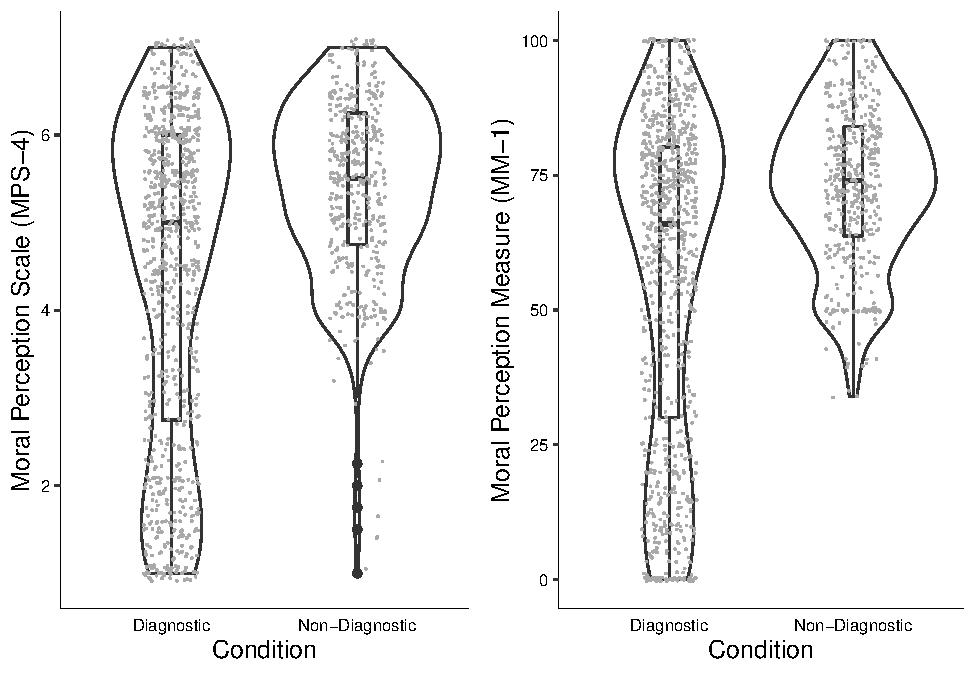
\includegraphics{pilot_1_files/figure-latex/pilot1bothconditionplot-1.pdf}
\caption{\label{fig:pilot1bothconditionplot}Pilot Study 1: Differences in moral perception depending on condition}
\end{figure}

We conducted a linear-mixed-effects model to test if condition influenced MM-1 responses. Our outcome measure was MM-1, our predictor variable was condition; we allowed intercepts and the effect of condition to vary across participants. Overall, the model significantly predicted participants responses, and provided a better fit for the data than the baseline model, \(\chi\)\textsuperscript{2}(2) = 924.82, \emph{p} \textless{} .001. Condition was a significant predictor in the model \(b\) = -8.22, \emph{t}(210.98) = -8.60, \emph{p} \textless{} .001, with the non-diagnostic descriptions being rated as more moral than the diagnostic descriptions, see Figure~\ref{fig:pilot1bothconditionplot}.

\hypertarget{refs}{}
\leavevmode\hypertarget{ref-grizzard_validating_2020}{}%
Grizzard, M., Fitzgerald, K., Francemone, C. J., Ahn, C., Huang, J., Walton, J., \ldots{} Eden, A. (2020). Validating the extended character morality questionnaire. \emph{Media Psychology}, \emph{23}(1), 107--130. \url{https://doi.org/10.1080/15213269.2019.1572523}

\leavevmode\hypertarget{ref-walker_better_2021}{}%
Walker, A. C., Turpin, M. H., Fugelsang, J. A., \& Białek, M. (2021). Better the two devils you know, than the one you don't: Predictability influences moral judgments of immoral actors. \emph{Journal of Experimental Social Psychology}, \emph{97}, 104220. \url{https://doi.org/10.1016/j.jesp.2021.104220}


\clearpage
\renewcommand{\listfigurename}{Figure captions}

\clearpage
\renewcommand{\listtablename}{Table captions}


\end{document}
